\section{Opis Modelu SI}\label{sec:opis-modelu-si}

Model sztucznej inteligencji został zaprojektowany w celu klasyfikacji zdjęć kości ośmiościennych k8 do jednej z ośmiu klas,
odpowiadających cyfrom od 1 do 8 na każdej ze ścianek.
Do implementacji modelu wykorzystano przede wszystkim moduł tensorflow oraz wchodzący obecnie w jego skład Keras,
który umożliwia łatwe tworzenie i trenowanie sieci neuronowych.

--- TODO --- linki z przypisami, cytowania dokumentacji Keras, Tensorflow

%% uselesss :(( \textit{Biblioteka Keras jest wygodnym opakowaniem (wrapperem) dla modeli DL używanych do oszacowań klasyfikacji lub regresji]} [Donald J. Norris, 2020 s. 355 wydanie APN PROMISE SA]


\subsection{Przygotowanie danych}\label{subsec:przygotowanie-danych}

Dane wejściowe zostały podzielone na zestawy treningowy i walidacyjny w proporcji 70:30.
W celu zwiększenia różnorodności danych treningowych zastosowano techniki augmentacji obrazów dostępne w klasie ImageDataGenerator, takie jak:

--- TODO --- cytowanie dokumentacji ImageDataGenerator

\begin{itemize}
    \item obrót o losowy kąt w zakresie do 90°,
    \item przesunięcia poziome i pionowe,
    \item transformacje perspektywiczne (shear) ,
    \item losowe powiększenia (zoom) .
\end{itemize}

\iffalse

\begin{figure}[H]
    \centering
    \begin{subfigure}[t]{0.32\linewidth}
        \centering
        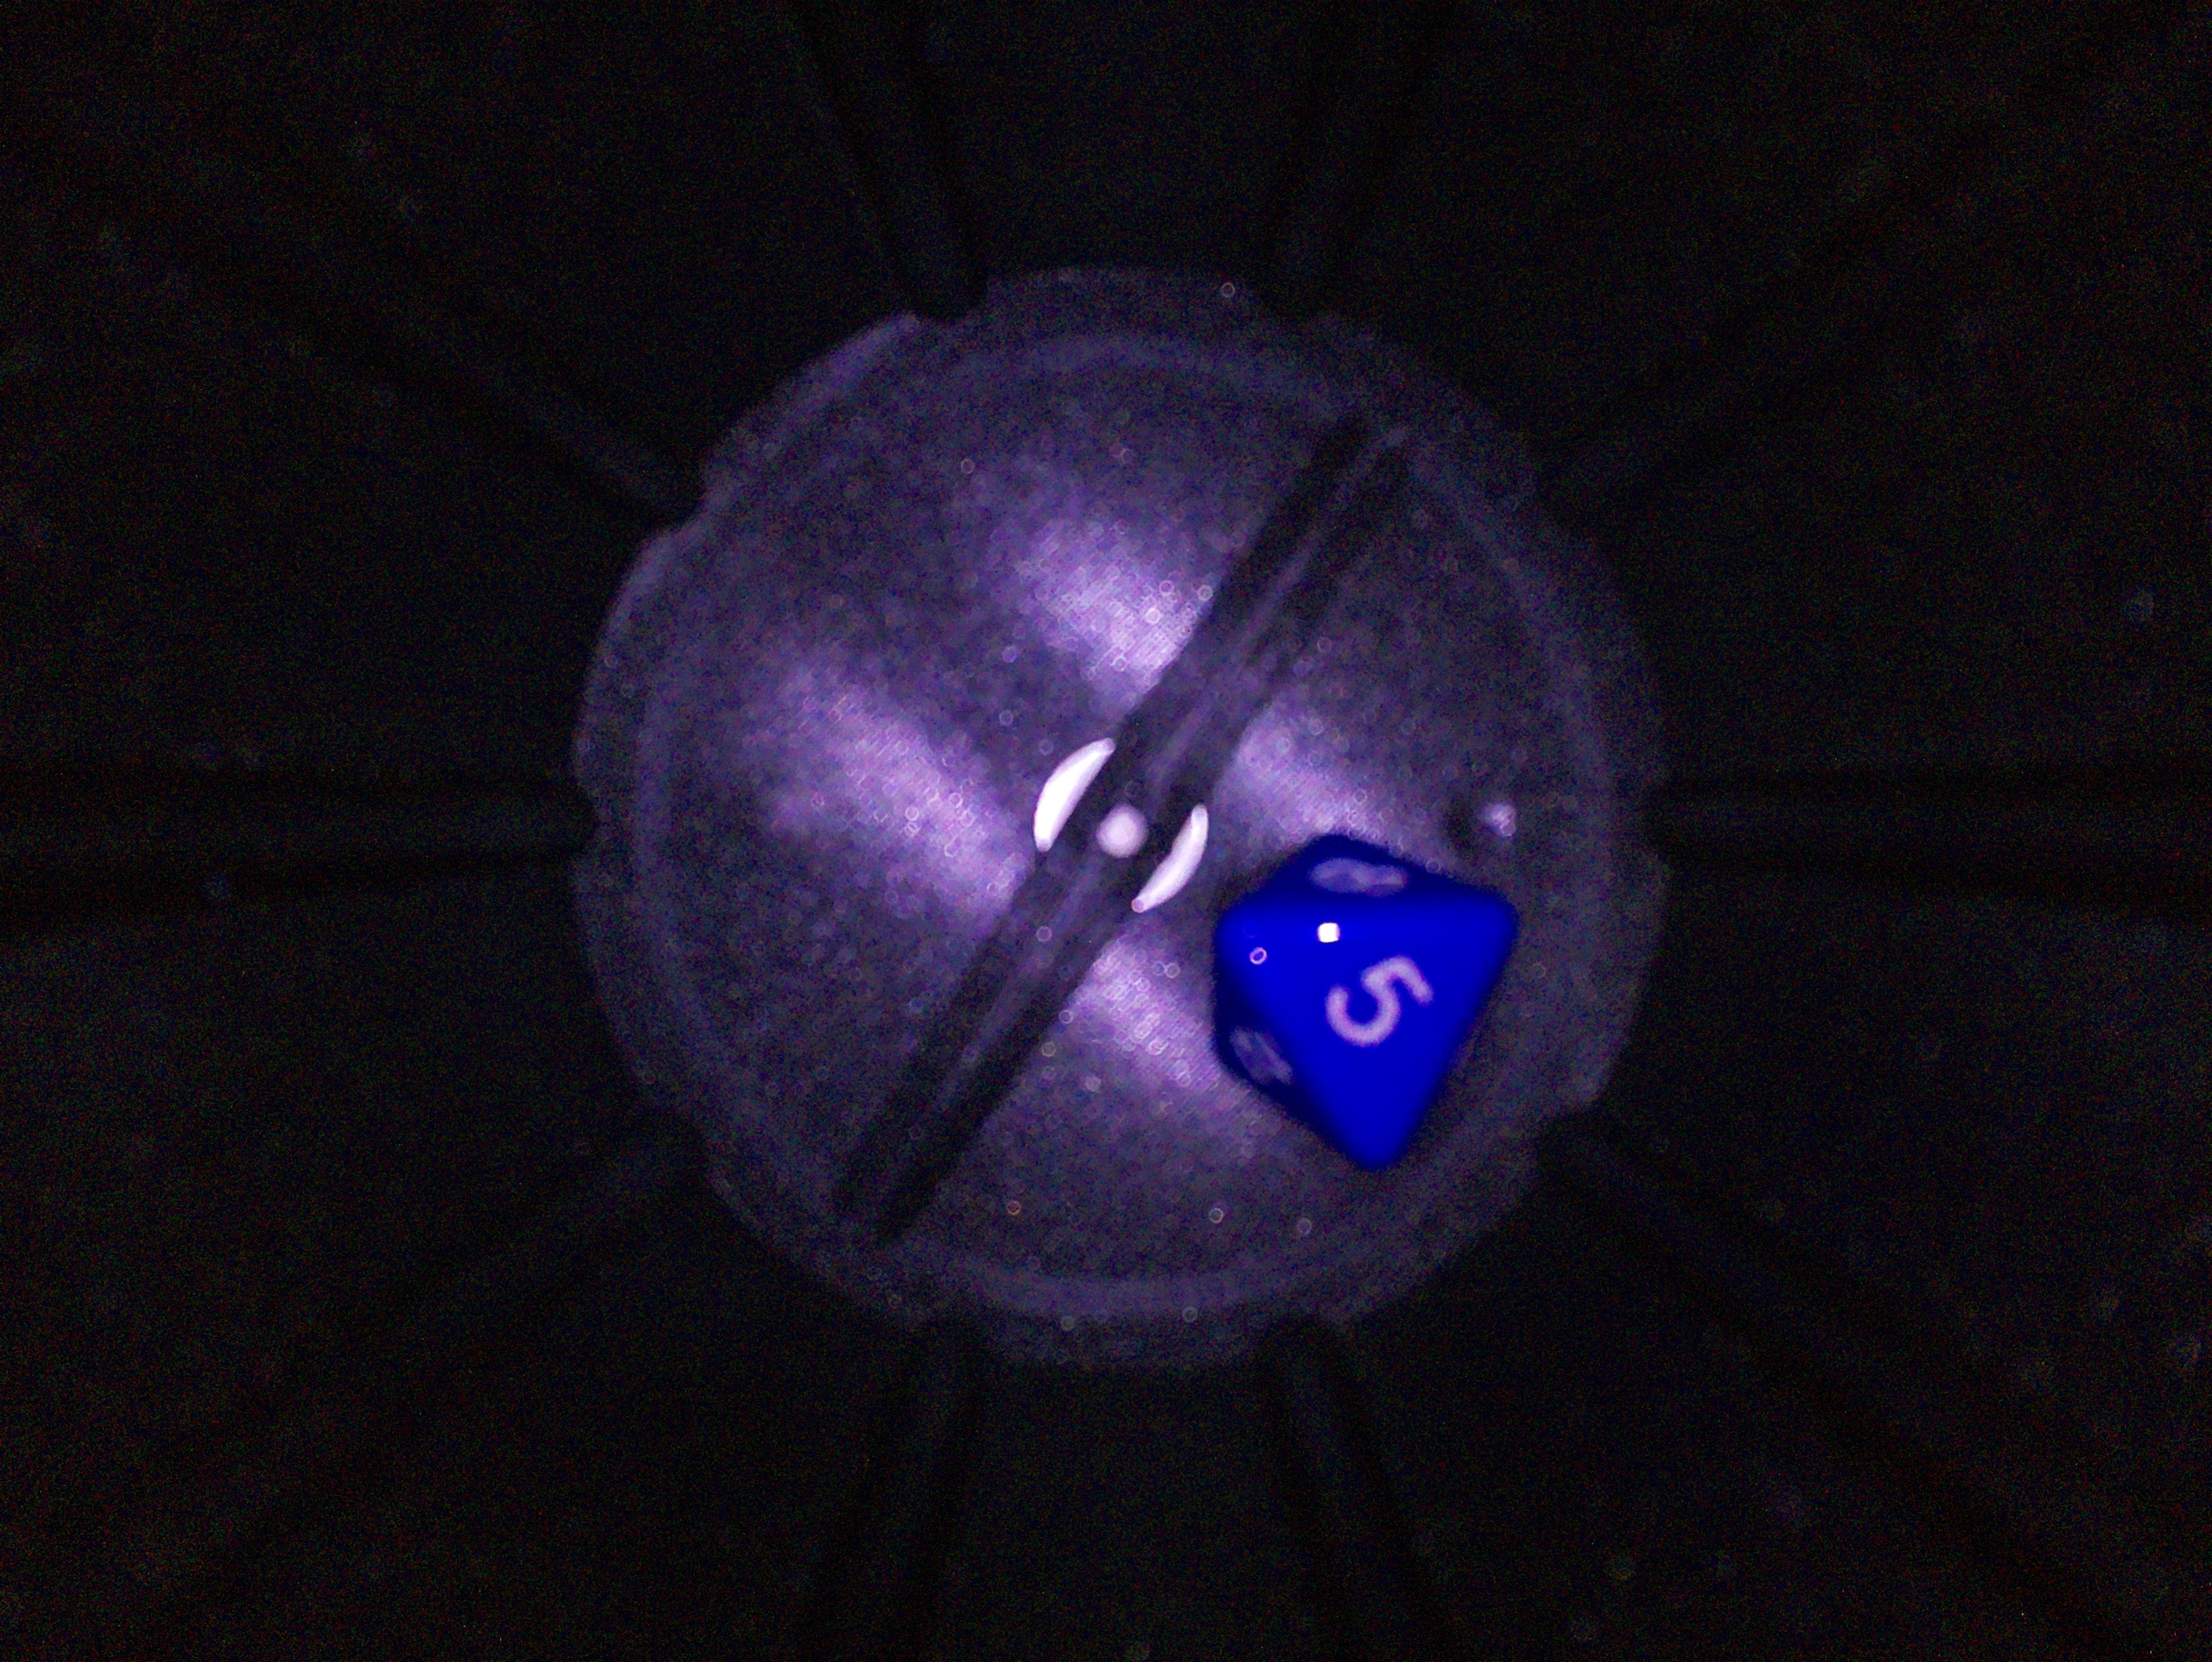
\includegraphics[width=\linewidth]{chapters/04-czytanie/figures/5_raw.jpg}
        \caption{Obraz surowy.}
        \label{fig:5raw}
    \end{subfigure}
    \hfill
    \begin{subfigure}[t]{0.32\linewidth}
        \centering
        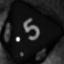
\includegraphics[width=\linewidth]{chapters/04-czytanie/figures/5_rotate.jpg}
        \caption{Obraz po obrocie.}
        \label{fig:5rotate}
    \end{subfigure}
    \hfill
    \begin{subfigure}[t]{0.32\linewidth}
        \centering
        \includegraphics[width=\linewidth]{chapters/04-czytanie/figures/5_move.jpg}
        \caption{Obraz po przesunięciu.}
        \label{fig:5move}
    \end{subfigure}

    \vspace{0.5cm} % Odstęp między wierszami obrazków

    \begin{subfigure}[t]{0.32\linewidth}
        \centering
        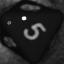
\includegraphics[width=\linewidth]{chapters/04-czytanie/figures/5_shear.jpg}
        \caption{Obraz po ścinaniu.}
        \label{fig:5shear}
    \end{subfigure}
    \hfill
    \begin{subfigure}[t]{0.32\linewidth}
        \centering
        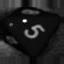
\includegraphics[width=\linewidth]{chapters/04-czytanie/figures/5_zoom.jpg}
        \caption{Obraz po powiększeniu.}
        \label{fig:5zoom}
    \end{subfigure}
    \hfill
    \begin{subfigure}[t]{0.32\linewidth}
        \centering
        \includegraphics[width=\linewidth]{chapters/04-czytanie/figures/5_combined.jpg}
        \caption{Obraz wynikowy.}
        \label{fig:5combined}
    \end{subfigure}

    \caption{Kolejne etapy przetwarzania obrazu, od surowego do wynikowego.}
    \label{fig:5processing}
\end{figure}

\fi

--- TODO --- dać obrazek surowy i każdą transformację. może też jakieś ich wszystkich złożenie, więc 6 obrazków?
dodatkowo, niech to będą obrazki 5 i potem porównanie lustrzanej 5 i 2 !!!


W szczególności należy zaznaczyć, że finalnie uniknięto początkowo przeoczonego błędu,
jakim jest tworzenie obrazów lustrzanych w wyżej wymienionych transformacjach, gdyż obrazy lustrzane
sprawiały że ścianki 2 oraz 5 były znacznie gorzej rozróżnialne przez wytrenowany model.

\subsection{Architektura modelu}\label{subsec:architektura-modelu}

--- TODO --- opis sieci splotowych CNN, czym są
opis warstwy gęstej, opisy funkcji aktywacji

Model jest wielowarstwową siecią splotową (ang. convolutional neural net (CNN))
składającą się z następujących elementów:

\begin{itemize}
    \item Warstwy wejściowej w rozmiarze 64 na 64 piksele, ale o jednym kanale (skala szarości)
    \item Trzech warstw splotowych z funkcją aktywacji ReLU:
    \begin{itemize}
        \item warstwa 1
        \item warstwa 2
        \item warstwa 3
    \end{itemize}
    \item Warstwy spłaszczającej (Flatten),
    \item Dwóch w pełni połączonych warstw (Dense), z których pierwsza również używa aktywacji ReLu,
a ostatnia używa funkcji aktywacji softmax do klasyfikacji na 8 klas.
\end{itemize}

\subsection{Użyte funkcje aktywacji}
--- TODO --- opis
\begin{itemize}
    \item ReLu
    \item Softmax
\end{itemize}

W przypadku zmiany kości na taką z inną liczbą ścianek, np.
na również rozważane w fazie koncepcyjnej kości czworościenną, sześciościenną, albo szesnastościenną,
ostatnia warstwa musiałaby również ulec odpowiedniej zmianie,
tak aby liczba neuronów odpowiadała liczbie ścianek na używanej kości.

\subsection{Trenowanie modelu}\label{subsec:trenowanie-modelu}

Model został nauczony z wykorzystaniem optymalizatora Adam,
funkcji strat sparse categorical crossentropy dostępnej w module tensorflow oraz metryki dokładności (ang. accuracy).
Proces trenowania obejmował 20 epok.
Na wejściu, model oczekiwał obrazu przedstawiającego wnętrze robota, wraz z kostką, znormalizowanego do przedziału $[0, 1]$.

--- TODO ---
cytowania dot.
- Adam
- sparse categorical crossentropy
- accuracy

\subsection{Wyniki}\label{subsec:wyniki}

Podczas trenowania osiągnięto następujące końcowe wyniki:

\begin{itemize}
    \item Dokładność na zbiorze treningowym: 0,9375
    \item Dokładność na zbiorze walidacyjnym: 1,0
    \item Strata na zbiorze treningowym: 0,0786
    \item Strata na zbiorze walidacyjnym: 0,0274
\end{itemize}

Wyniki zostały również zwizualizowane na wykresach przedstawiających zmianę dokładności i straty w trakcie trenowania.

\begin{figure}[H]
    \centering
    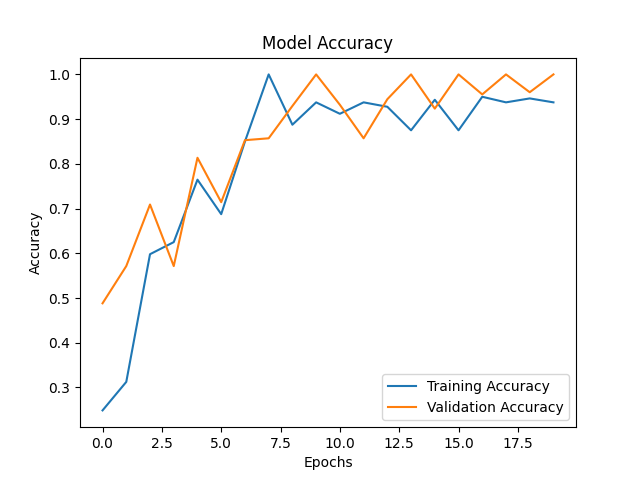
\includegraphics[width=0.7\textwidth]{chapters/04-czytanie/figures/ModelAcc1}
    \caption{Wykres dokładności modelu.}
    \label{fig:ModelAcc}
\end{figure}

\begin{figure}[H]
    \centering
    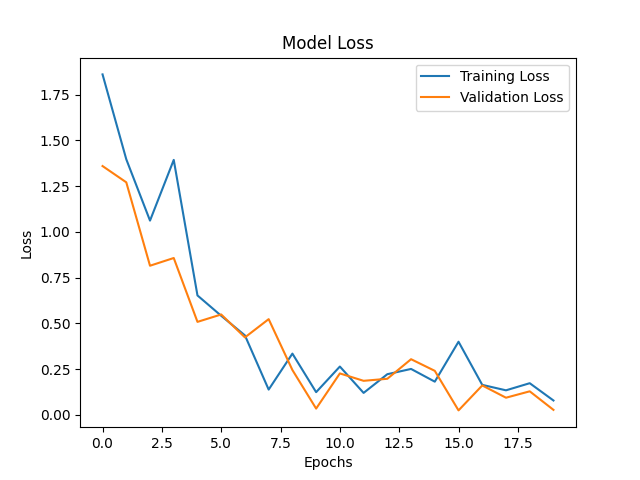
\includegraphics[width=0.7\textwidth]{chapters/04-czytanie/figures/ModelLoss1}
    \caption{Wykres straty modelu.}
    \label{fig:ModelLoss}
\end{figure}

Model został zapisany w formacie \texttt{keras} i jest gotowy do użycia w systemie rozpoznawania liczb na ośmiościennej kości,
opisanym w kolejnej sekcji.


\subsection{Podsumowanie}

--- TODO ---
if needed, to be checked i guess
